\item Problem 4.2

\begin{center}
    \begin{tabular}{|c|c|c|c|}
        \hline
        Sources & Weight\% & Flow (kg/h) & Load (kg/h) \\
        \hline
        Absorber I & 5 & 5100 & 255 \\
        Acid Tower & 10 & 10200 & 1020 \\
        \hline
    \end{tabular} 
    
    \begin{tabular}{|c|c|c|c|}
        \hline
        Sinks & Weight\% & Flow (kg/h) & Load (kg/h) \\
        \hline
        Absorber II & 14 & 1400 & 196 \\
        Primary Tower & 25 & 9100 & 2275 \\
        \hline
    \end{tabular} 
\end{center}

Plot sink and sources composite lines.

\begin{align*}
    \intertext{Sink lines}
    \text{Load} &= 0.05 \cdot \text{Flow} \text{, until 5100 kg/h} \\
    \text{Load} &= 0.1 \cdot \left(\text{Flow} - 5100\right) + 255 \text{, until 15300 kg/h} \\
    \intertext{Source lines; guess x-intercept}
    \text{Load} &= 0.14 \cdot \left(\text{Flow} - \text{x-intercept}\right) \text{, until x-intercept + 1400 kg/h} \\
    \text{Load} &= 0.25 \cdot \left(\text{Flow} - \text{x-intercept} - 1400\right) \\ 
    & + 0.14 \cdot \left(\text{x-intercept} + 1400\right) \text{, until x-intercept + 1400 kg/h} \\ 
    & \text{, until x-intercept + 10500 kg/h} \\
\end{align*}

Plot the lines and vary the x-intercept until the sink and source lines intersect.

\begin{center}
    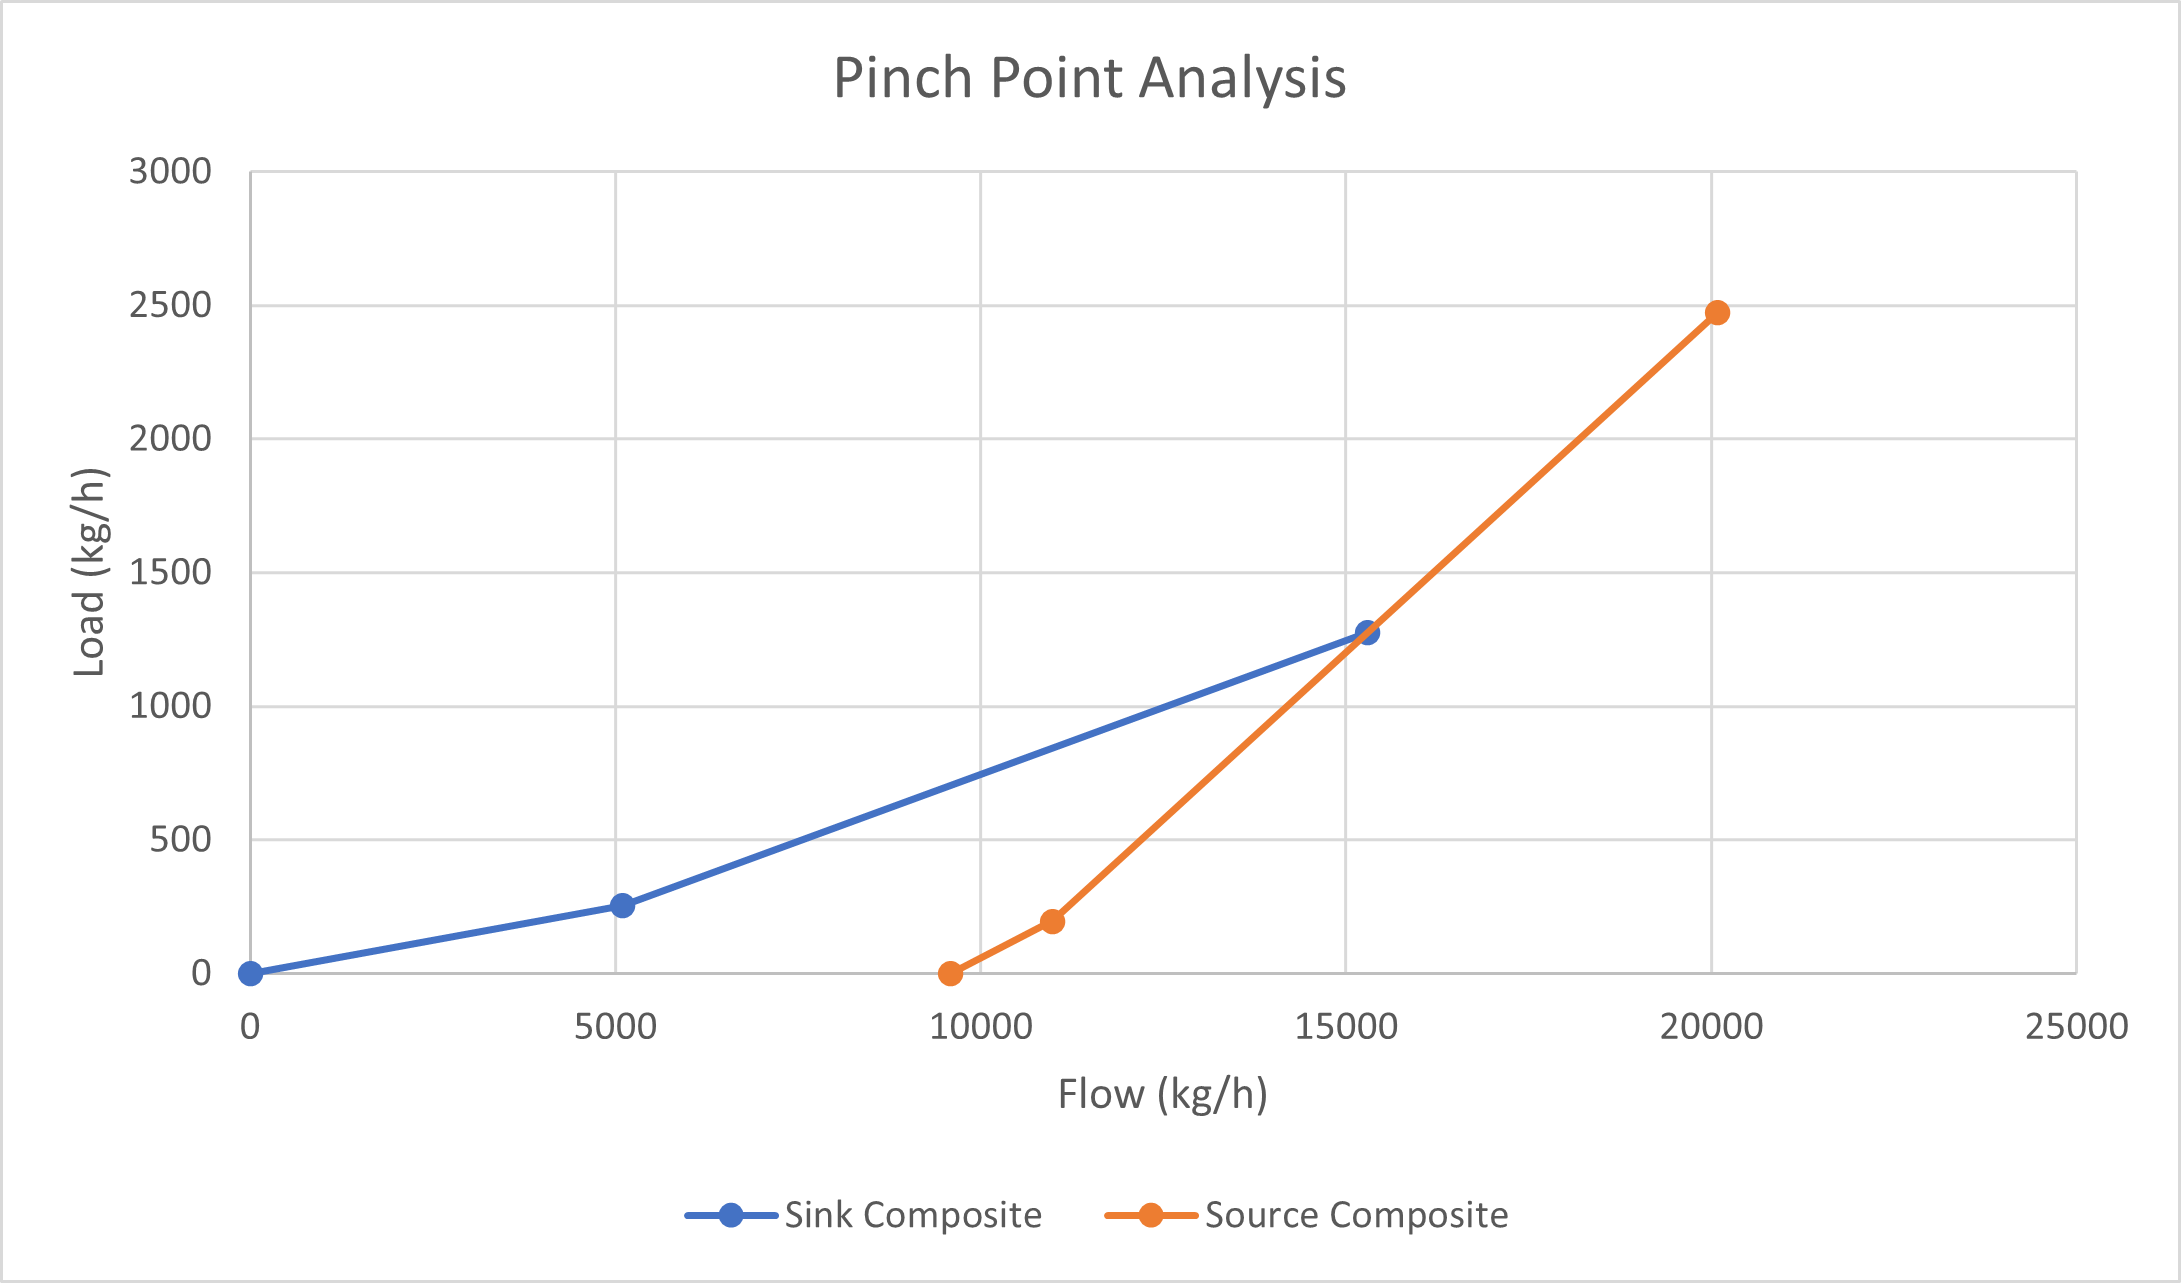
\includegraphics[width=0.8\textwidth]{assets/p2.png}
\end{center}

The pinch point came at an x-intercept of 9584. The target fresh acetic acid usage is 9584 kg/h and the target minimumm discharge is 4784 kg/h.

One possible way of achieving this process is by taking the discharge streams and mixing a portion of it with the fresh acetic acid feed, and then sending the mixture to the respective units.

Another way of integrating the process is by reducing the fresh feed rates to the Absorber II and the Primary tower. Then, feed the entirety of the discharge from the Absorber I to the Absorber II. Then, send the rest of the recyclable discharge to the Primary Tower.

The final way of integrating this process is by reducing the fresh feed rates to the Absorber II and the Primary tower. Then, combine the waste discharge streams and make of the rest of the required acetic acid to the Absorber II and the Primary tower with the combined discharge.